\documentclass{ctexart}
\usepackage{graphicx} % Required for inserting images
\usepackage{amsmath}
\usepackage{booktabs}
\usepackage[left=2.5cm,right=2.5cm,top=2.5cm,bottom=2.5cm]{geometry}
\begin{document}
\section{实验目的}

\begin{enumerate}
    \item 复习低通、高通、带通电路、带阻电路的频率特性
    \item 学习使用Multisim设计和测试低通、高通、带通电路、带阻电路
    \item 学习使用Multisim软件的交流分析功能
    \item 复习电路谐振的原理与观察方法
\end{enumerate}
\section{实验原理}
\subsection{RC串联电路的频域分析}
对于已经达到正弦稳态的电路,由于用经典法进行时域分析计算量较大,所以我们常常采用频域分析法。
\begin{figure}[h]
    \centering
    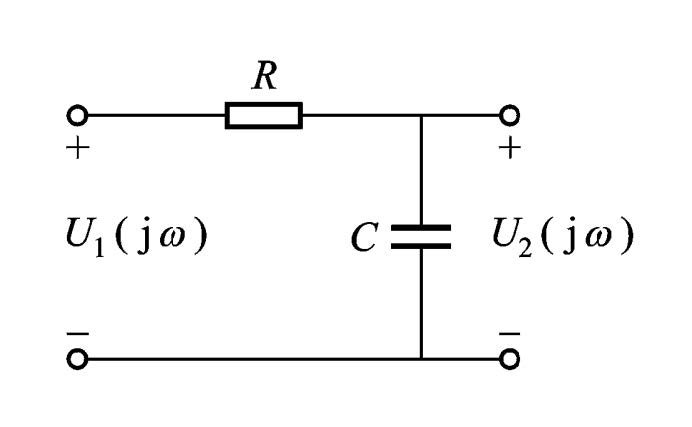
\includegraphics{pic/RC电路图.jpg}
    \caption{RC电路图}
    \label{fig:RC串联电路图}
\end{figure}
对于图\ref{fig:RC串联电路图}所示的电路,将所有的电路量变换至频域。设电源的有效值为$U_s$,则电源的相量为$\Dot{U_s}=U_s\angle 0^\circ $,则电流相量为
\begin{equation}
    \Dot{I}=\dfrac{\Dot{U_s}}{R+\dfrac{1}{j\omega C}}
\end{equation}
电容上的电压为
\begin{equation}
    \Dot{U_C}=\Dot{I}\cdot \dfrac{1}{j\omega C}=\dfrac{U_s}{1+j\omega CR}
\end{equation}
其有效值为
\begin{equation}
    U_C=\dfrac{U_s}{\sqrt{1+(\omega CR)^2}}
\end{equation}
根据截止频率的定义,当输出电压为电压源的$\dfrac{\sqrt{2}}{2}$倍时,对应的电源频率称为截止频率$f_0$,此时$\varphi(j\omega)=45\circ$。代入定义,得到截止频率的计算公式
\begin{equation}
    \omega CR =1
\end{equation}
即
\begin{equation}
    f_0=\dfrac{1}{2\pi CR}
\end{equation}
通过定性分析发现,当频率升高时,电容上的电压变小,电阻上的电压变大。利用这一特性我们可以设计高通和低通电路。
\subsection{RLC串联电路的谐振现象}
一般而言,RLC串联电路(图\ref{fig:RLC串联电路图})中电流和电源电压是不同相的,但是,通过调节电容电感参数和电源频率,我们可以使得电流和电源电压同相,此时称该电路发生了谐振。
\begin{figure}[h]
    \centering
    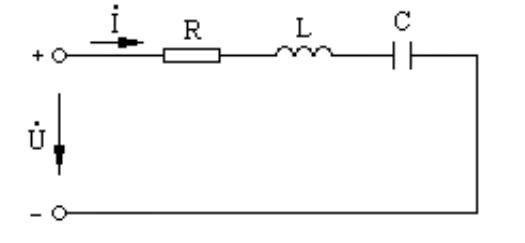
\includegraphics{pic/RLC串联电路图.jpg}
    \caption{RLC串联电路图}
    \label{fig:RLC串联电路图}
\end{figure}
从第五版《电路》(邱关源著)的对应章节得知,此时电感和电容满足
\begin{equation}
    \omega L= \dfrac{1}{\omega C}
\end{equation}
若固定电容和电感参数,则需调节电源频率为
\begin{equation}
    f_0=\dfrac{1}{2 \pi \sqrt{LC}}
\end{equation}
谐振电路有许多特殊的性质。比如,此时的电阻电压达到最大值;电感和电容上的电压始终等大反向。我们可以利用这些性质设计带通、带阻电路。
\section{实验内容}
\subsection{用Multisim 分析功能测试一阶RC 低通电路的频率特性}
设计电路图如图\ref{fig:实验5-1电路图}所示
\begin{figure}[ht]
    \centering
    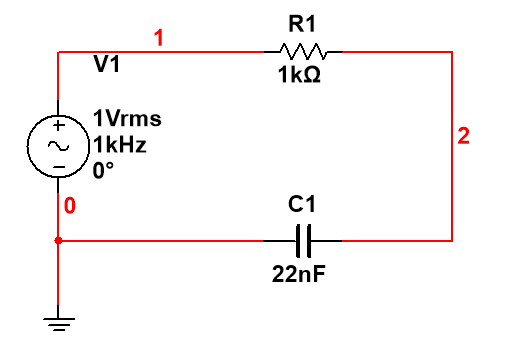
\includegraphics{pic/实验5-1电路图.png}
    \caption{实验5-1电路图}
    \label{fig:实验5-1电路图}
\end{figure}
对V2进行交流分析,得到如图所示的幅频和相频图像
\begin{figure}[h]
    \centering
    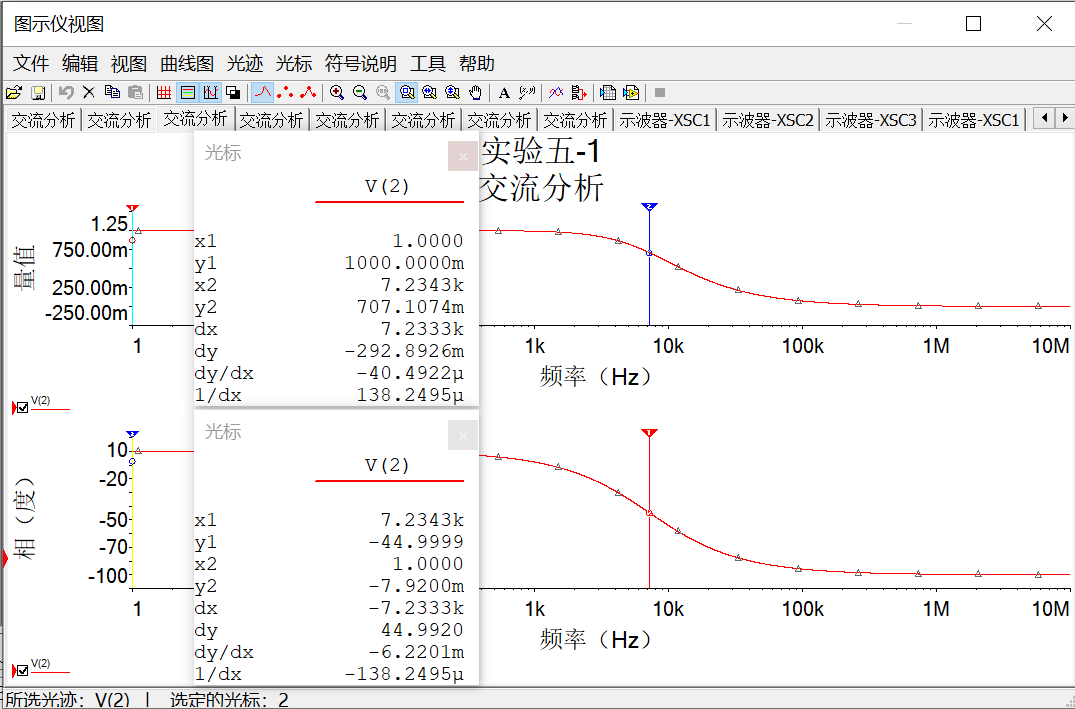
\includegraphics[scale=0.5]{pic/实验5-1,相频特性.png}
    \caption{5-1交流分析}
    \label{fig:5-1交流分析}
\end{figure}
将光标移到使V2大约为电源有效值的0.707倍,此时的频率对应为$f_0=7.2343kHz$,这与通过理论计算得到的值非常接近。下面我们用表\ref{tab:一阶RC低通电路频率特性测量}给出在不同$f$取值下的幅值与相值
\begin{table}[h]
    \centering
    \begin{tabular}{|c|c|c|c|c|c|c|c|}
        \hline
        ~ & 0.01$f_0$ &  0.1$f_0$ & 0.5$f_0$ & $f_0$ & 5$f_0$ & 10$f_0$ & 100$f_0$ \\ \hline
        |H(j$\omega$)| & 999.950m & 995.0372m & 894.4274m & 707.1074m & 196.1166m &99.5040m & 9.9995m \\ \hline
        $\varphi(j\omega)({}^\circ)$ & -572.9378m& -5.7106 & -26.5650 & -44.9999 & -78.6900 & -84.2894 & -89.4271  \\ 
        \hline
        
    \end{tabular}
    \caption{一阶RC低通电路频率特性测量}
    \label{tab:一阶RC低通电路频率特性测量}
\end{table}
\subsection{设计一阶高通电路,用Multisim 分析测试其频率特性}
根据实验原理部分的分析,可以用一个RC串联电路设计高通电路。考虑到手中已有的电路元件有限,我们使用$C=22nF$的电容进行设计。
根据公式
\begin{equation}
    f_0=\dfrac{1}{2 \pi CR}
\end{equation}
可以反推出电阻的计算公式
\begin{equation}
    R=\dfrac{1}{2 \pi f_0 C}
\end{equation}
代入数据可得,电阻的阻值为$R=8038.1286\Omega$,考虑到实际阻值不便取这一值,我们取为8000$\Omega$。下面用Multisim来仿真测试。

设计如图\ref{fig:实验5-2电路图}所示的电路图
\begin{figure}[ht]
    \centering
    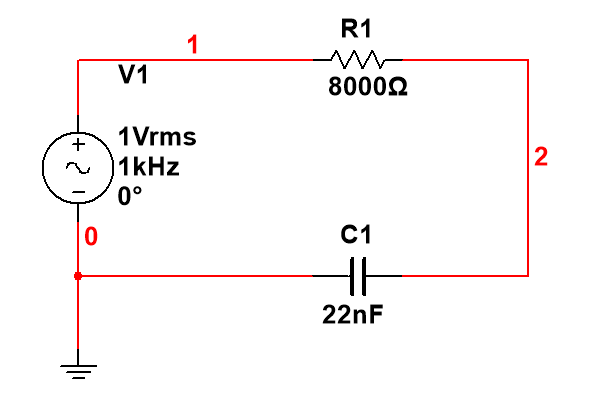
\includegraphics[scale=0.5]{pic/实验5-2电路图.png}
    \caption{实验5-2电路图}
    \label{fig:实验5-2电路图}
\end{figure}
交流分析界面如图\ref{fig:实验5-22交流分析}所示
\begin{figure}[ht]
    \centering
    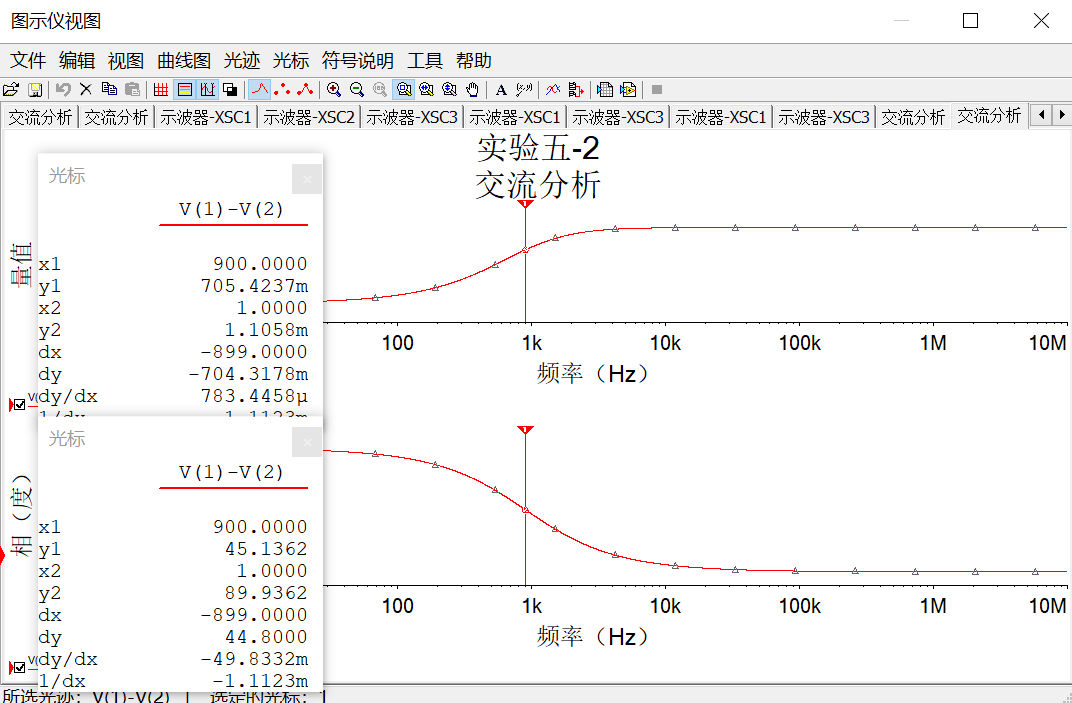
\includegraphics[scale=0.5]{pic/实验5-2,相频特性.png}
    \caption{实验5-2交流分析}
    \label{fig:实验5-22交流分析}
\end{figure}
代入R=8000$\Omega$的实际电阻值,算出理论截止频率为$f_0=904.289Hz$。可以看到,输入光标的纵坐标值为900Hz,此时的输出电压(即R上的电压,V1-V2)为705mV左右,基本符合要求。
\subsection{将内容2、1 电路串联,用Multisim 测试其电路的频率特性,并进行说明分析。}
串联电路图如图\ref{fig:实验5-3电路图}所示
\begin{figure}[h]
    \centering
    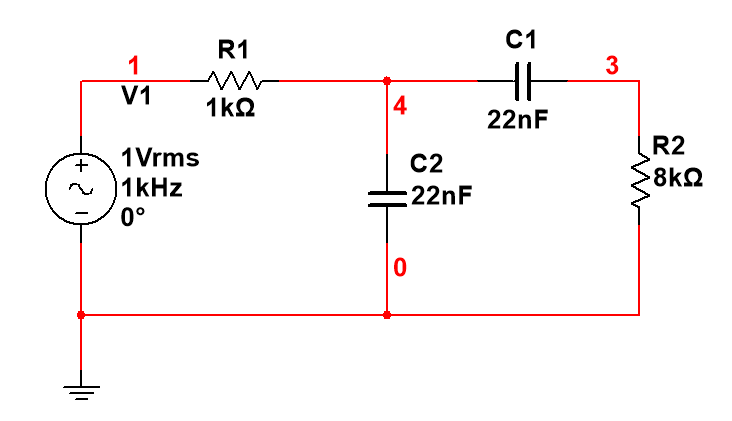
\includegraphics[scale=0.5]{pic/实验5-3电路图.png}
    \caption{实验5-3电路图}
    \label{fig:实验5-3电路图}
\end{figure}
一个电路的输出作为第二个电路的输入,经过理论计算得到截止频率为
\begin{equation}
    f_0=\dfrac{1}{2\pi \sqrt{R_1R_2C_1C_2}}
\end{equation}
代入值算出该电路的截止频率为$f_0=2557.7168Hz$。
\begin{figure}[h]
    \centering
    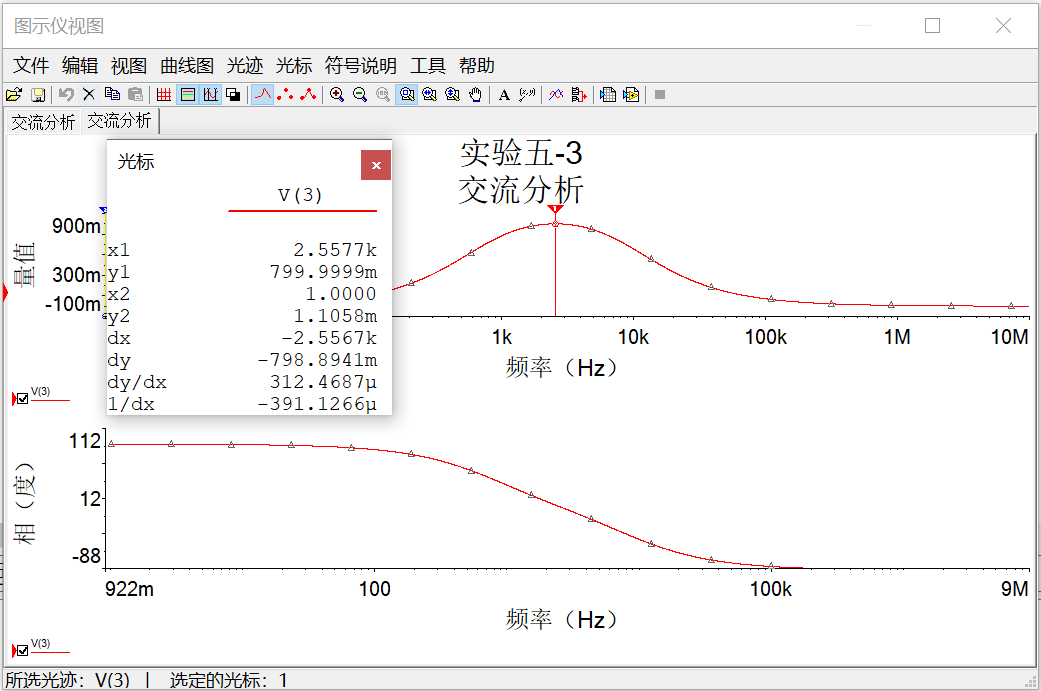
\includegraphics[scale=0.5]{pic/实验5-3相频特性.png}
    \caption{实验5-3相频特性}
    \label{fig:实验5-3相频特性}
\end{figure}
图\ref{fig:实验5-3相频特性}的交流分析界面显示,理论与仿真结果吻合程度较好。
\subsection{RLC串联谐振电路测量}
\subsubsection{按照所给条件设计电路图}
在Multisim上设计的电路如图\ref{fig:RLC谐振电路图}所示
\begin{figure}[h]
    \centering
    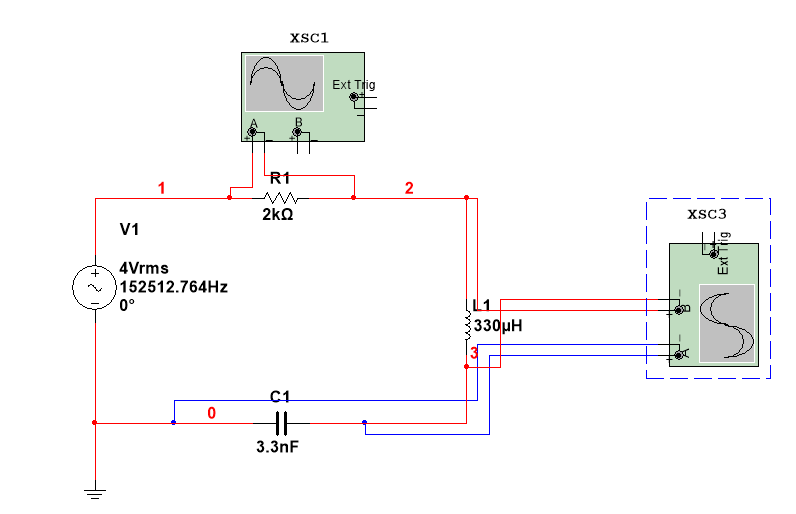
\includegraphics[scale=0.5]{pic/RLC谐振电路图.png}
    \caption{RLC谐振电路图}
    \label{fig:RLC谐振电路图}
\end{figure}
\subsubsection{利用Multisim仿真,测量三个元件上的电压在谐振点上的波形}
设置电源频率为谐振频率$f_0=152512.764Hz$。进行频域分析,得到图\ref{fig:实验5-4频域分析}所示的界面
\begin{figure}[h]
    \centering
    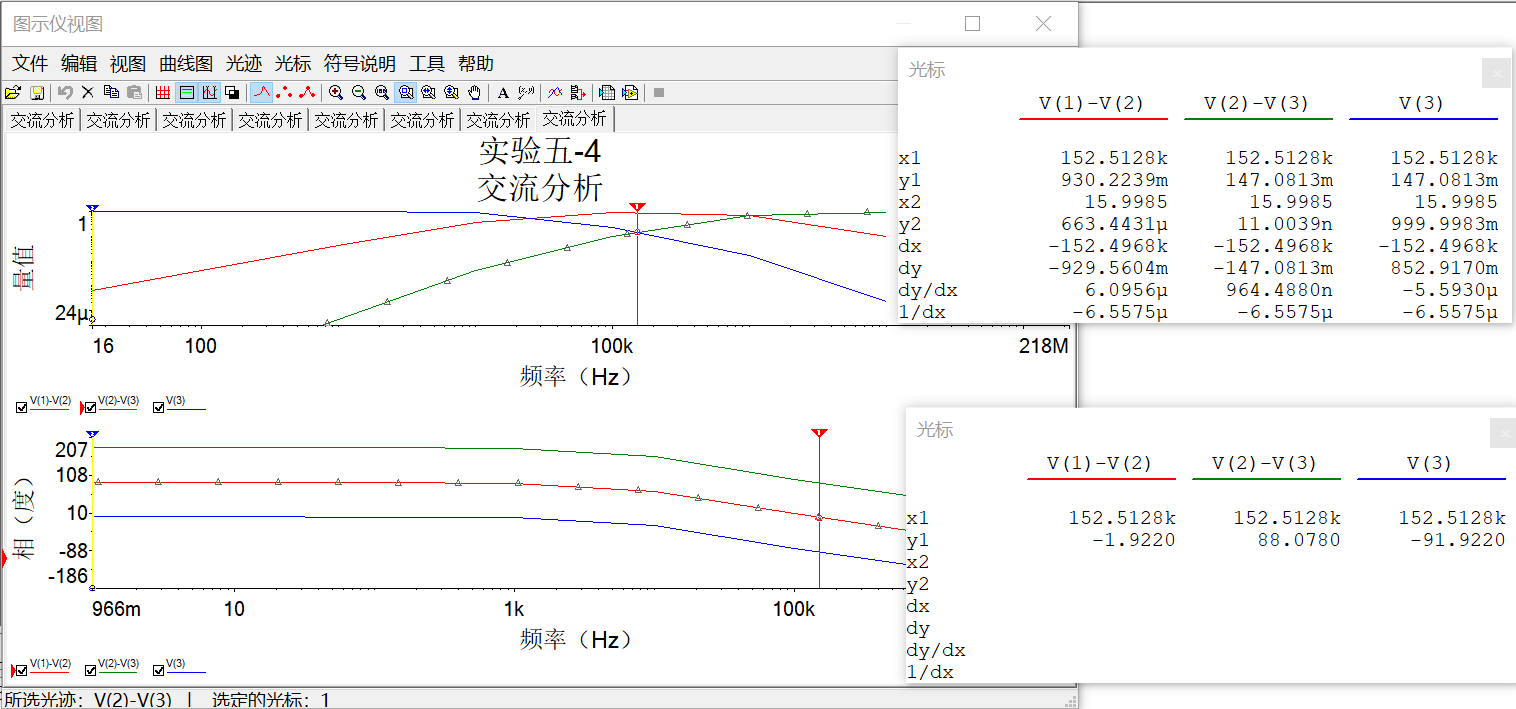
\includegraphics[scale=0.5]{pic/实验5-4相频特性.png}
    \caption{实验5-4频域分析}
    \label{fig:实验5-4频域分析}
\end{figure}
可以看到,随着频率的升高,电容上的电压逐渐降低,电感上的电压逐渐升高,而电阻上的电压先升后降。这是由于电容和电感的阻抗随着频率的改变而改变。在频域使用分压原理进行定性分析,与仿真结果吻合。

接着,测量电容和电感上的输出电压的波形,如图\ref{fig:RLC谐振示波器界面}所示
\begin{figure}[h]
    \centering
    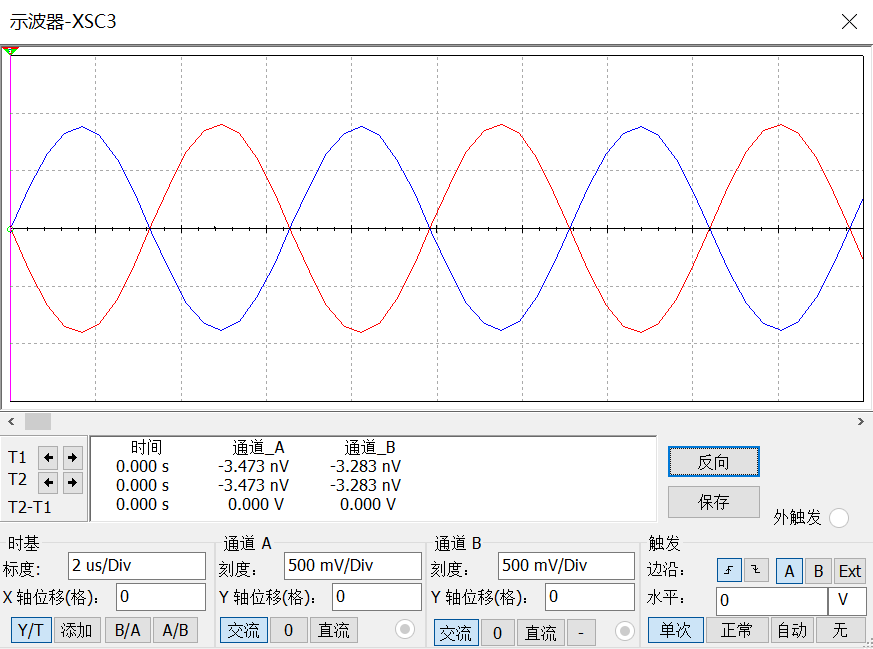
\includegraphics[scale=0.5]{pic/RLC谐振示波器.png}
    \caption{RLC谐振示波器界面,蓝色指示电容,红色指示电感}
    \label{fig:RLC谐振示波器界面}
\end{figure}
可以看到,在谐振点上,电感和电容上的电压始终等大反向(达到正弦稳态后),因为此时有两者阻抗相等:
\begin{equation}
    \omega L =\dfrac{1}{\omega C} 
\end{equation}
而电感电压始终超前电阻90度,电容滞后90度,所以电感和电容相位相差180度,再加上阻抗值相等的条件,就得到了等大反向的结果。
\subsubsection{说说如何利用RLC串联电路实现带通和带阻电路}
既然在谐振点上,电容和电感电压等大反向,则若设置输出电压$U_O$为二者电压之和,那么$U_O$几乎为零,获得了“阻断”的效果。与此同时,电阻上的输出电压达到最大值。综上,将输出电压设置在电阻两端,可以获得带通电路;设置在电容电感串联的两端,可以获得带阻电路。其中,通带和阻带都在谐振点附近。
\subsubsection{搭建实物电路,再现谐振现象,并测量三个元件上的波形}
搭建如图所示的电路图
\begin{figure}[h]
    \centering
    \includegraphics[scale=0.07]{pic/RLC实物电路图.jpg}
    \caption{RLC实物电路图}
    \label{fig:RLC实物电路图}
\end{figure}
测量电阻上的电压。调节函数发生器的频率为理论谐振频率,发现电阻上的电压(CH2)与输入电压(CH1)几乎同相,相位差CH1-CH2为-2.74$^\circ$。为了验证是否该电压频率就是谐振点,我们逐渐调节电源频率,发现无论如何调节,输出电压与输入电压的相位差总是增大,且输出电压的有效值也单调减小,说明初始调节的电压就是谐振点。其示波器的示数如图所示
\begin{figure}[h]
    \centering
    \includegraphics[scale=0.07]{pic/RLC电阻.jpg}
    \caption{RLC实物电路中,电源与电阻的波形图}
    \label{fig:RLC实物电路中,电源与电阻的波形图}
\end{figure}
保持电源频率不变,再测量电感上的电压。通过示波器图\ref{fig:RLC实物电路中,电源与电感的波形图}我们发现,电源有效值仍为3.86V,而电感上的电压为641.2mV。
\begin{figure}[h]
    \centering
    \includegraphics[scale=0.07]{pic/RLC电感.jpg}
    \caption{RLC实物电路中,电源与电感的波形图}
    \label{fig:RLC实物电路中,电源与电感的波形图}
\end{figure}
为了验证这一结果的正确性,我们计算电路的理论品质因数
\begin{equation}
    Q=\dfrac{\omega L}{R}=\dfrac{1}{\omega RC}=0.1581
\end{equation}
而品质因数的实际值为
\begin{equation}
    Q=\dfrac{U_L}{U_s}=0.1661
\end{equation}
误差在4.8\%左右,属于允许范围内。
保持电源频率不变,再测量电容上的电压。
\begin{figure}[h]
    \centering
    \includegraphics[scale=0.07]{pic/RLC电容.jpg}
    \caption{RLC实物电路中,电源与电容的波形图}
    \label{fig:RLC实物电路中,电源与电容的波形图}
\end{figure}
通过示波器图\ref{fig:RLC实物电路中,电源与电容的波形图}我们发现,电源有效值仍为3.86V,而电感上的电压为653.6mV。
品质因数的实际值为
\begin{equation}
    Q=\dfrac{U_L}{U_s}=0.1693
\end{equation}
误差在6.6\%左右,属于允许范围内。
\subsubsection{实物电路现象与仿真结果对比并分析原因}
实验误差的来源有很多。比如电子元件本身有误差,其参数不可能像理论值一样准确,特别是电感本身的电阻,对实验结果的影响较大;电路搭建过程中,电路的导线、引脚的连接情况也会影响示数;再比如,示波器的读数也不稳定,我们只是截取了某个瞬间的读数作为实验数据来记录。
\section{实验仪器}
\begin{enumerate}
    \item 鼎阳SDS1000X
    \item 万用表UT803
    \item 信号源SDG1000X
\end{enumerate}
\section{思考题}
(1)Multisim 仿真电路中输入信号源起什么作用,改变信号源的参数对测试结果有无影响?

输入信号源起提供激励函数的作用。改变信号源的幅度,影响输出电压的大小。改变信号源的频率,根据输出电路是高通、低通、带通还是带阻,会影响输出电压的值。

(2)试写出判定 RLC 串联电路处于谐振状态的三种实验方法。

\begin{enumerate}
    \item 测量输入电压和电阻上的电压波形,当二者相位差为0时,电路谐振
    \item 测量电容和电感上的输出电压,当二者相差180度时,电路谐振
    \item 测量电容(或电感)和电阻上的电压,当二者相差90度的时候,电路谐振(电容滞后,电感超前)
\end{enumerate}
(3)RLC 串联谐振电路实物实验中,信号源输出信号幅度该如何选择?测量过程中,信号源信号幅度有没有变化?

选择信号源幅度为4V(RMS),不要太大也不要太小。测量过程中,发现信号源幅度在3.86V左右,总是小于设定值。推测可能是由于传输线损耗和测量误差造成的。

(4)在谐振频率点及谐振频率左右,电路的特性有什么变化?

电路在谐振频率点上时,回路电流和信号源同相,此时电阻上的电压达到最大值,整个电路呈现电阻的特性。当频率小于谐振频率时,电路显示出电容的特性(容性阻抗);当频率大于谐振频率时,电路显示出电感的特性(感性阻抗)。

\section{参考文献}
无
\end{document}
